\documentclass{article}
\usepackage{graphicx}
\usepackage{amsmath}
\numberwithin{figure}{section}
\usepackage{indentfirst}
\documentclass{article}
\usepackage{hyperref}

\title{Analysis of Interplanetary Trajectories via the Method of Patched Conics}
\author{Ewan Alvarez - ela7827}
\date{23 December 2024}

\begin{document}

\maketitle

\section{Hohmann Transfers}

When considering the transfer of a spacecraft from one orbit to another, whether it be to another celestial body or otherwise, one must first consider a \textit{Hohmann transfer}. A Hohmann transfer is an idealized maneuver for moving a spacecraft between two coplanar, concentric circular orbits. This is achieved via two precise velocity changes, the difference of which is referred to as \(\Delta v\) or notated as \(\Delta v\), with the first increase allowing for escape from the first orbit into an interplanetary elliptical orbit, called the \textit{Hohmann transfer ellipse}, before another velocity increase to enter the second circular orbit. 

The radial position where you leave on the first orbit becomes the \textit{periapsis} of the Hohmann transfer ellipse and where you arrive is the \textit{apoapsis}. It is additionally worth noting that if two elliptical orbits are being considered instead of circular, there is an option to leave from the periapsis or apoapsis of orbit 1, arriving at the apoapsis or periapsis, respectively, of orbit 2.

Due to the only two changes in velocity, Hohmann transfers are incredibly efficient, requiring little propellant; however, they consequently result in a significantly longer travel time. Nonetheless, considering Hohmann transfers provides useful insight into how total energy changes during interplanetary travel, as well as how predetermined orbits can be leveraged to propel a spacecraft with very little additional energy changes.

\begin{figure}
    \centering
    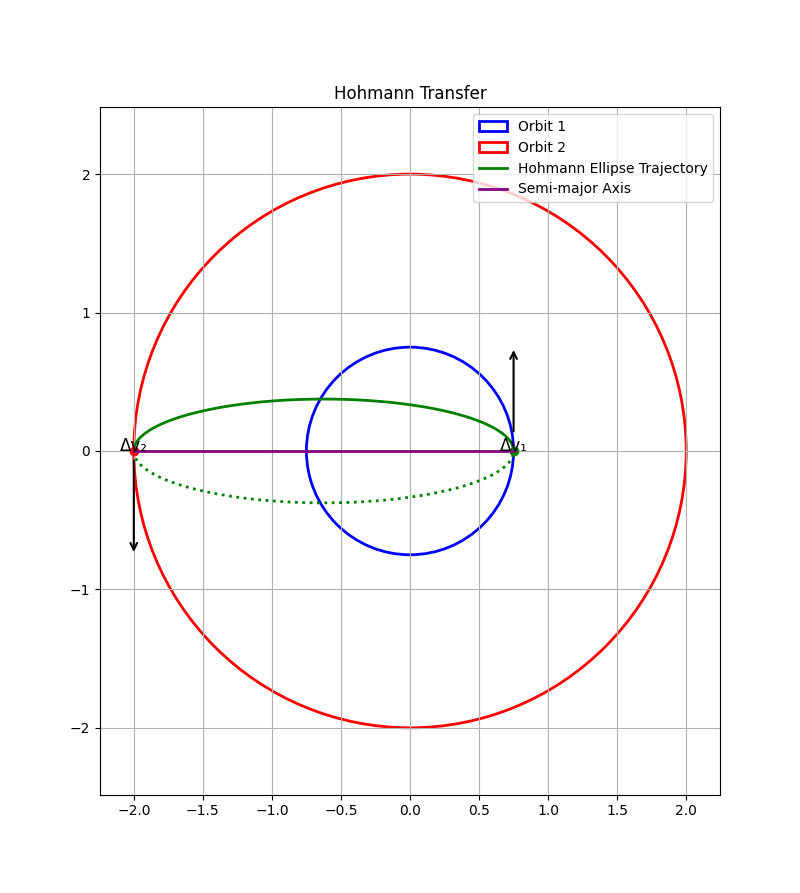
\includegraphics[width=0.5\linewidth]{hohman.png}
    \caption{Hohmann Transfer from \texttt{matplotlib}}
    \label{fig:enter-label}
\end{figure}

Hohmann transfers can be generalized into four steps:

\subsection*{1.1 Choose the axis of the initial and final orbit:}
Because the orbits in Hohmann transfers are circular, this can be a straight line through the first orbit going to the second orbit, i.e., a line from the center of the circle to any radial position on the second orbit. This axis can be calculated via the equation:

\[
a = \frac{r_0 + r_1}{2}
\]

where:
\begin{itemize}
    \item \(r_0\) is the radius of the initial orbit,
    \item \(r_1\) is the radius of the final orbit,
    \item \(a\) is the semi-major axis of the transfer ellipse.
\end{itemize}

\subsection*{1.2 Calculate the velocities of each circular orbit:}
The orbital velocity for a circular orbit is given by:

\[
v_{c} = \sqrt{\frac{\mu_{\text{planet}}}{r}}
\]

where:
\begin{itemize}
    \item \(\mu_{\text{planet}}\) is the standard gravitational parameter of the central body
    \item \(r\) is the radius of the orbit.
\end{itemize}

\subsection*{1.3 Calculate the initial and final velocities of the elliptical orbit:}
These velocities correspond to:
\begin{itemize}
    \item The velocity when you start the elliptical orbit after the first velocity change (\(v_p\) at periapsis), and
    \item The velocity at the end of the elliptical orbit when the second velocity change is required (\(v_a\) at apoapsis).
\end{itemize}

The velocities can be calculated using the \textit{vis-viva equation}:

\[
v = \sqrt{\mu_{\text{planet}} \left( \frac{2}{r} - \frac{1}{a} \right)}
\]

where:
\begin{itemize}
    \item \(v\) is the relative speed of the two bodies,
    \item \(r\) is the distance between the bodies' center of masses,
    \item \(a\) is the semi-major axis of the transfer orbit.
\end{itemize}

The change in velocity (\(\Delta v\)) is then:

\[
\Delta v = |v_c - v|
\]

\subsection*{1.4 Calculate the transfer time:}
The time required for the transfer is half the orbital period of the transfer ellipse, given by:

\[
t = \pi \sqrt{\frac{a^3}{\mu_{planet}}}
\]

where:
\begin{itemize}
    \item \(t\) is the transfer time,
    \item \(a\) is the semi-major axis of the transfer ellipse,
    \item \(\mu_{planet}\) is the standard gravitational parameter of the central body.
\end{itemize}
\section{Energy Changes}
\subsection{2.1 First Orbit}
It has been established that in order to escape the first orbit, an increase in velocity is required. In addition, to enter the second orbit, a much larger orbit than the interplanetary elliptical orbit, another increase in velocity is required. Whenever velocity increases, the total energy of the orbit becomes less negative (i.e., increases), but it remains negative for a bound orbit. If the velocity reaches or exceeds escape velocity, the total energy becomes zero or positive, indicating an unbound orbit. If we are considering a bound circular orbit around the first planet, we could graph the effective potential energy of the system via the equation:

\[
U_{\text{eff}}(r) = -\frac{GMm}{r} + \frac{L^2}{2mr^2}
\]

where:
\begin{itemize}
    \item \(U_{\text{eff}}(r)\) is the effective potential energy as a function of \(r\),
    \item \(G\) is the gravitational constant,
    \item \(M\) and \(m\) are the masses of the central body and the smaller body, respectively,
    \item \(r\) is the radial distance,
    \item \(L\) is the angular momentum.
\end{itemize}

The spacecraft would therefore be in a bound orbit between the two points that intersect the curve underneath the line of total energy. The graph of effective potential of the orbit is shown in Figure 2.1.

\begin{figure}[h]
    \centering
    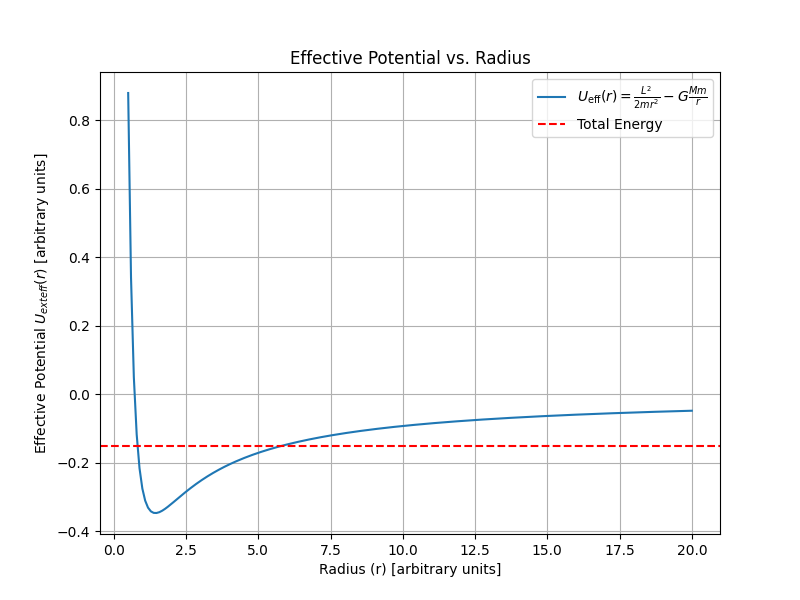
\includegraphics[width=0.5\linewidth]{potent1.png}
    \caption{Effective Potential Energy of the First Orbit from \texttt{matplotlib}}
    \label{fig:enter-label}
\end{figure}
\subsection{2.2 Hohmann Transfer Ellipse Orbit}
If we now consider the elliptical portion of the Hohmann transfer, velocity has increased so the graph in Figure 2.1 should be shifted up. The total energy of the graph is less negative and our angular momentum is higher due to an increase in velocity, so the "well" shape that indicates the closed orbit should be wider, additionally supporting the fact that we are in an elliptical orbit. This is shown in Figure 2.2.

\begin{figure}
    \centering
    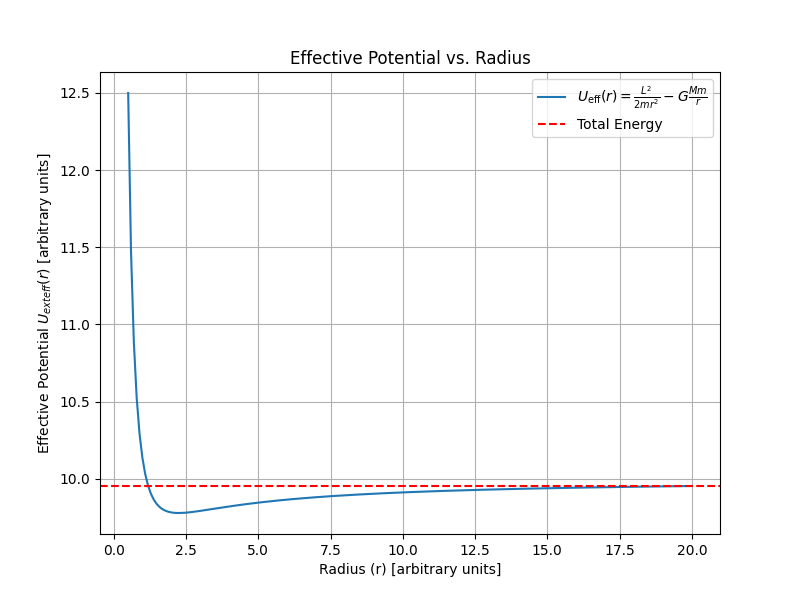
\includegraphics[width=0.5\linewidth]{elliptical.png}
    \caption{Effective Potential of the Hohmann Transfer Elliptical Orbit from \texttt{matplotlib}}
    \label{fig:enter-label}
\end{figure}

\subsection{2.3 Second Orbit}
Entering the second orbit requires another increase in velocity in order to match the circular orbit. Because the orbit is circular, the line of total energy that we have denoted in Figure 2.1 and Figure 2.2 would be lower, as the radius of the larger circle is still smaller than the semi-major axis of the Hohmann transfer ellipse. In other words, the spacecraft is more tightly bound in this more stable circular orbit, however, angular momentum does increase so the graph should be moderately flat. There should be a sweet spot in graphing the effective potential of this stage, in which the "well" shape is noticeably deep---deeper than the elliptical orbit---and the portion of the curve underneath the line of total energy should be fairly flat---flatter than the first orbit, less flat than the elliptical orbit.

\section{Spheres of Influence}
Three primary celestial bodies affect the trajectory of a spacecraft moving in interplanetary space: the one from which it is departing, the one it is seeking to arrive at, and the sun. Despite the enormous mass difference between the sun and every other body in our solar system, Newton's law of gravity shows that force due to gravity is inversely proportional to the square of the distance, meaning that when close enough to another planet, that planet's force of gravity far exceeds that of the sun's. This region in which the planet's gravitational attraction is greater than the sun's is referred to as that planet's \textit{sphere of influence} (SOI). 

When considering interplanetary trajectories, the borders of each sphere of influence, i.e. the border of the SOI of the departure planet and the border of the SOI of the arrival planet, each mark the point when the trajectory is now primarily affected by a different mass. Using Newton's law of gravity, it can be found that the radius of a planet's SOI can be given by the equation:

\[
r_{SOI}=R\sqrt{\frac{m_{p}}{m_{s}}}
\]
where:
\begin{itemize}
    \item \(R\) is the distance from the center of the sun to the planet,
    \item \(m_{p}\) is the mass of the given planet,
    \item \(m_{s}\) is the mass of the sun.
\end{itemize}

\section{Method of Patched Conics}
Having established spheres of influence and Hohmann transfers, we can begin to consider the method of patched conics (now considering elliptical planetary orbits instead of circular) which refers to the literal “patching” of three conic sections: the elliptical transfer orbit, the hyperbolic departure trajectory, and the hyperbolic arrival trajectory. More specifically, we analyze three frames: the two body frames of the planets and the sun’s frame. The elliptical trajectory is determined as it is for Hohmann transfers, via a tweaked version of the vis viva equation, in the sun’s frame, while the changes in departure and arrival velocities required to enter the elliptical orbits of each planet is calculated within the frame of that planet. The method of patched conics consequently makes the process of three frame shifts streamlined.

\subsection*{4.1 Depature}
As previously discussed, to leave the orbit of the first planet, the velocity of the spacecraft needs to be increased, resulting in a hyperbolic trajectory as viewed in planet 1’s frame. The speed which the spacecraft needs to be raised by is called the \textit{hyperbolic excess velocity}, or \(v_\infty\), notated as \(v_\infty\). If not for this excess amount of velocity, the departure speed, that is the speed to leave the sphere of influence of the planet, would approach zero as it approached the radius of the sphere of influence. Therefore, upon leaving the sphere of influence, the leftover, or excess, velocity you would have would be \(v_\infty\).

From the vis-viva equation, the following equation for \(v_\infty\) can be derived:

\[
v_\infty = \sqrt{\frac{\mu_{\text{sun}}}{R_1}} \left( \sqrt{\frac{2 R_2}{R_1 + R_2}} - 1 \right)
\]

where:
\begin{itemize}
    \item \(\mu_{\text{sun}}\) is the standard gravitational parameter of the Sun,
    \item \(R_1\) is the radial distance of the initial orbit measured from the center of mass of planet 1,
    \item \(R_2\) is the radial distance of the final orbit measured from the center of mass of planet 1,
    \item \(v_\infty\) is the hyperbolic excess velocity.
\end{itemize}

or, in vector form:

\[
\vec{v_\infty}=\vec{V_{\text{D}}}-\vec{V_1}
\]
where:
\begin{itemize}
    \item \(\vec{V_{\text{D}}}\) is the minimum departure velocity,
    \item \(\vec{V_1}\) is the relative velocity of the planet.
\end{itemize}

\begin{figure}
    \centering
    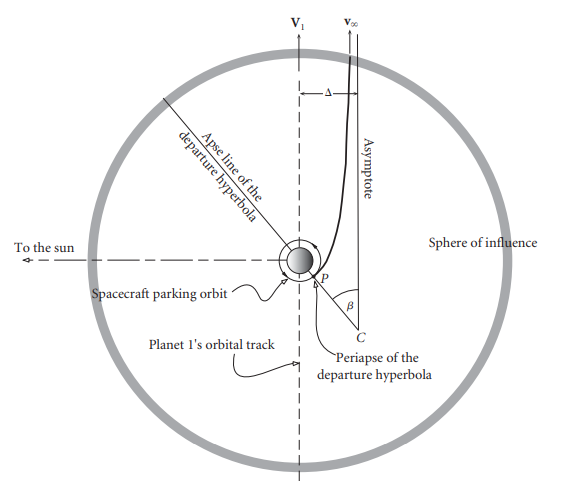
\includegraphics[width=0.5\linewidth]{v infinite.png}
    \caption{Hyperbolic Trajectory from \textit{Orbital Mechanics for Engineering Students} by Howard D. Curtis}
    \label{fig:enter-label}
\end{figure}

A visualization of the hyperbolic departure from a circular is shown in Figure 3.1, highlighting the body frame analysis required for the departure. It is worth noting that, as shown in the figure, the asymptote to which \(v_\infty\) approaches is parallel to \(\vec{V_1}\) as is standard in Hohmann transfers. This all means that the spacecraft, using the velocity given by its orbit of the planet, as well as the velocity which it is already traveling at, gets ahead of the planet and, combining the gravitational attraction of the sun and the hyperbolic trajectory which it is traveling at, will arc into the orbit of the second planet. Choosing the periapsis to be the point at which you depart is useful for more than one reason:
\begin{enumerate}
    \item The maximum orbital speed is achieved at the periapsis, according to Kepler's Second Law
    \item The distance from the COM of the planet is trivial to get
    \item As a consequence, the eccentricity and angular momentum are also trivial to get
    \[e = 1 + \frac{r_p v_\infty^2}{\mu_{\text{planet}}}\]
    \[L = r_p \sqrt{v_\infty^2 + \frac{2 \mu_{\text{planet}}}{r_p}}\]
\end{enumerate}

Having the eccentricity will tell us \(\beta\), shown in Figure 4.1, which is the angle which our delta-v maneuver must occur, and angular momentum allows us to calculate the delta-v required to put the spacecraft into hyperbolic departure trajectory. The total change in velocity, \(\Delta v\) can be calculated as follows:

\[
\Delta v = v_p - v_c = v_c \left( \sqrt{2 + \left( \frac{v_\infty}{v_c} \right)^2} - 1 \right)
\]

where:
\begin{itemize}
    \item \(\Delta v\) is the change in velocity, or delta-v,
    \item \(v_p\) is the velocity at periapsis,
    \item \(v_c\) is the velocity in the circular orbit velocity,
    \item \(v_\infty\) is the hyperbolic excess velocity.
\end{itemize}

while \(\beta\) can be calculated with the eccentricity:
\[
\beta = \cos^{-1}\left( \frac{1}{e} \right)
\]
\subsection*{4.2 Arrival}
As touched on, when you are out of the SOI of the first orbit, you are at a speed of \(v_\infty\) only, meaning when you enter the SOI of the second orbit you are at that speed. Because the spacecraft is arriving at a speed less than the speed of the planet itself, an increase in velocity is required to enter the orbit. Therefore, our new equation for \(v_\infty\) is given by:
\[
v_(\infty)=\vec{V_2}-\vec{V_A}
\]
At this point, the goal of the mission will change when the delta-v burn must occur. If the goal is simply a fly-by, our \(\Delta\), i.e. the distance between the asymptote \(v_\infty\) approaches and \(\vec{V_2}\), there is far more leeway in when the delta-v maneuver must occur, as, if no great impact with the planet occurs, the spacecraft will simply continue past the periapsis and continue at a different angle still at velocity \(v_\infty\). In order to impact the planet, our \(\Delta\) must be aimed such that the hyperbola's periapsis roughly equals the radius of the planet. \(\Delta\) can be given by the following expression:
\[
\Delta = r_p \left( 1 + \frac{2\mu_\text{planet}}{r_p v_\infty^2} \right)
\]

where:
\begin{itemize}
    \item \(\Delta\) is the parameter (replace with specific meaning, if applicable),
    \item \(r_p\) is the periapsis distance (of both the elliptical planetary orbit and hyperbolic trajectory),
    \item \(\mu_\text{planet}\) is the standard gravitational parameter,
    \item \(v_\infty\) is the hyperbolic excess velocity.
\end{itemize}
Now, if we wanted to enter an elliptical orbit of eccentricity \textit{e} around a planet, our delta-v maneuver would have to occur at the periapsis. This allows us to calculate the required velocity at that point, given by:
\[
v_{\text{p,hyp}} = \sqrt{v_\infty^2 + \frac{2\mu_\text{planet}}{r_p}}
\]
We can also find the velocity corresponding to the capture orbit by applying with our previous equation for \(v_c\) to an ellipse:
\[
v_{\text{p,capture}} = \sqrt{\frac{\mu_\text{planet}(1 + e)}{r_p}}
\]
Therefore, the delta-v required is simply the difference:
\[
\Delta v = v_{\text{p,hyp}} - v_{\text{p,capture}} = \sqrt{v_\infty^2 + \frac{2\mu_\text{planet}}{r_p}} - \sqrt{\frac{\mu_\text{planet}(1 + e)}{r_p}}
\]
Now, using useful substitutions and taking the derivative twice, it can be found that the minimum delta-v required to enter an elliptical orbit is:
\[
\Delta v = v_\infty \sqrt{\frac{1 - e}{2}}
\]
and the corresponding \(\Delta\) required for this \(\Delta v\) is
\[
\Delta = \sqrt{\frac{2}{(1 - e)}}{r_p}
\]
From this equation, we can conclude that extremely eccentric elliptical capture orbits, i.e. those that are almost parabolic, have a much smaller margin of error.
\section{Non-Hohmann Interplanetary Trajectories}

Rather unsurprisingly, real life procedures for space travel are not as idealized as simplified Hohmann transfers make them out to be. Nonetheless, the method of patched conics can still be applied to three-dimensional trajectories, mostly subbing in vectors for what were previously not vectors. This process is practically identical to solving Lambert's problem, having a very similar algorithm. 
\subsection*{Lambert's Problem}
Let's consider a problem requiring that we send a spacecraft from planet 1 to planet 2 in a given time \(t_\text{12}\). We are given a starting \(\vec{R_1}\), i.e. the position of the planet with respect to the sun, at this time \(t_\text{12}\) as well as an ending \(\vec{R_2}\) at time \(t_12\)+t, some additional time t. With this and some information about the planets alone, we are able to determine the transfer trajectory's six orbital elements required for this transfer, the six shown in Figure 5.1: 
\begin{enumerate}
    \item h - specific angular momentum
    \item i - inclination (determines trajectory type, prograde or retrograde)
    \item \(\Omega\) - Right ascension of the ascending node - determines what quadrant our trajectory will be relative to the sun
    \item e - eccentricity, determines type of conic section, e > 1 is a hyperbola, e = 1 is a parabola, 0 < e < 1 is an ellipse
    \item \(\omega\) - argument of perigee - determines where in the orbit our spacecraft will approach the central body (i.e. tells us the angular position of the periapsis)
    \item \(\theta\) - true anomaly - tells us the current position of our spacecraft in its orbit, as well as the periapsis
\end{enumerate}

\begin{figure}
    \centering
    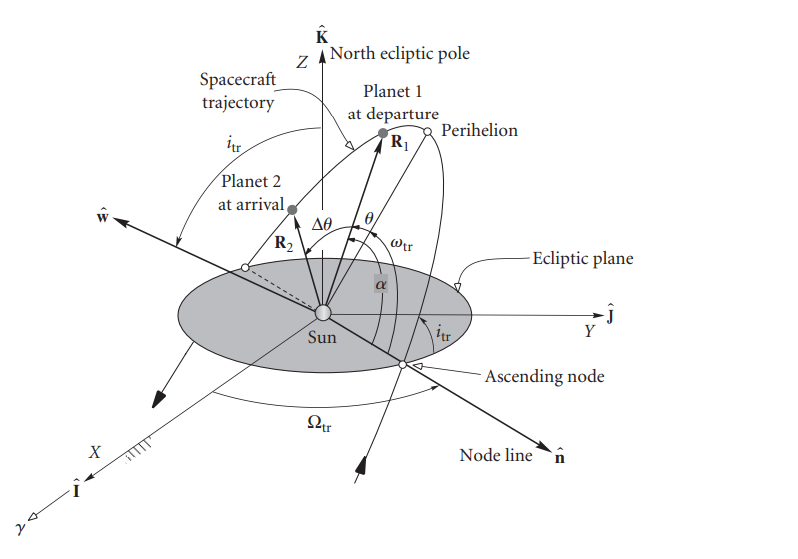
\includegraphics[width=0.5\linewidth]{orbital elements.png}
    \caption{Heliocentric Orbital Elements of a 3D Transfer Trajectory from \textit{Orbital Mechanics for Engineering Students} by Howard D. Curtis}
    \label{fig:enter-label}
\end{figure}

This is also incredibly useful in determining whether or not such a mission is possible given this amount of time, or given these positions, allowing us to solve for whatever is required to make them possible.

First, we must choose a desired trajectory type: prograde or retrograde. Prograde refers to to an objects spin being in the same direction as its trajectory, while retrograde refers to an objects spin opposing its trajectories. This decision will simply affect some criteria about the change in true anomaly, which is the orbital element that defines the position of our spacecraft. For the sake of simplicity, let us choose a prograde trajectory, additionally assuming that the z-component of the cross product of \(\vec{R_1}\) and \(\vec{R_2}\) is greater than 0. With this in mind, the change in true anomaly is given by the expression:
\[
\Delta \theta = \cos^{-1} \left( \frac{\mathbf{R_1} \cdot \mathbf{R_2}}{R_1 R_2} \right)
\]
Let us also define a unitless constant A, which is useful in calculations:
\[
A = \frac{\sin \Delta\theta \, R_1 R_2}{1 - \cos \Delta\theta}
\]

It is also now worth defining two functions referred to as Stumpff functions. These are functions used to analyze this kind of problem, whether it be launch trajectories or escape trajectories. They are primarily defined by the following infinite series:
\[
S(z) = \sum_{k=0}^{\infty} \frac{(-1)^k z^k}{(2k + 3)!}
\]
\[
C(z) = \sum_{k=0}^{\infty} \frac{(-1)^k z^k}{(2k + 2)!}
\]
Given a finite z value, these series will always converge absolutely---another reason why they are used for this kind of problem.

Next, we must solve a system of equations a generalized form of z in order to determine the type of conic section or orbit is.

\[
F(z) = \left( \frac{y(z)}{C(z)} \right)^{\frac{3}{2}} S(z) + A \left( \sqrt{y(z)} - \sqrt{\mu} \,\Delta t \right)
\]
\[
F'(z) = 
\begin{cases} 
\left( \frac{y(z)}{C(z)} \right)^{\frac{3}{2}} \left( \frac{1}{2z} \left( C(z) - \frac{3}{2} \frac{S(z)}{C(z)} \right) + \frac{3}{4} \frac{S(z)^2}{C(z)}\right) + \frac{A}{8} \left( \frac{3 S(z)}{C(z)} \sqrt{y(z)} + A \sqrt{\frac{C(z)}{y(z)}} \right) & \text{for } z \neq 0, \\
\frac{\sqrt{2}}{40} y(0)^{\frac{3}{2}} + \frac{A}{8} \left( \sqrt{y(0)} + A \sqrt{\frac{1}{2y(0)}} \right) & \text{for } z = 0.
\end{cases}
\]
\[
z_{i+1} = z_i - \frac{F(z_i)}{F'(z_i)}
\]
For z>0, our orbit is a hyperbola, for z=0 our orbit is a parabola, and for z<0 our orbit is an ellipse.

Having solved for the sign of z, we can solve for y(z). y(z) is a substituted function taken from an expression for the universal anomaly, which is a sort-of universal tie in for all hyperbolic and elliptical trajectory equations. By solving for y(z), however, we can solve for the Lagrange coefficients f, g, and \(\dot{g}\), which will allow us to solve for \(\vec{v_1}\) and \(\vec{v_2}\) in a later step. The equation we must solve for y(z) is as follows: 
\[
y(z) = r_1 + r_2 + A \frac{z S(z) - 1}{\sqrt{C(z)}}
\]
Finally, we can solve for the lagrange coefficients, which will directly give us the velocity vectors via the following equations:
\[
f = 1 - \frac{y(z)}{r_1}
\]
\[
g = A \sqrt{\frac{y(z)}{\mu}}
\]
\[
\dot{g} = 1 - \frac{y(z)}{r_2}
\]
Then we can find \(\vec{v_1}\) and \(\vec{v_2}\):
\[
\vec{v_1} = \frac{1}{g} \left( \vec{R_2} - f \vec{R_1}\right)
\]
\[
\vec{v_2} = \frac{\dot{g}}{g} \vec{R_2}
\]
\subsection*{Orbital Elements}
As with solving Lambert's Problem, this is process if purely algorithmic. There are 10 steps:
\begin{enumerate}
    \item Find the radial velocity:
    \[
v_r = \frac{\vec{r} \cdot \vec{v}}{r}
\]
    \item (1/6) Find the specific angular momentum, magnitude and vector:
    \[
\vec{h} = \vec{r} \times \vec{v}
\]
\[
h = \sqrt{\vec{h} \cdot \vec{h}}
\]
    \item (2/6) Calculate the inclination:
    \[
i = \cos^{-1} \left( \frac{\vec{h} \cdot \hat{z}}{|\vec{h}|} \right)
\]
    \item Find the vector that defines the node line and its magnitude (the node is point at which the spacecraft trajectory intersects the Earth's elliptical plane, the node line is the vector starting from the sun and intersecting the node)
\[
\vec{N} = \hat{K} \times \vec{h} =
\begin{vmatrix}
\hat{i} & \hat{j} & \hat{k} \\
0 & 0 & 1 \\
h_X & h_Y & h_Z
\end{vmatrix}
\]
\[
N = \sqrt{\vec{N} \cdot \vec{N}}
\]
    \item (3/6) Calculate the right ascension fo the ascending node:
    \[
\Omega = \cos^{-1} \left( \frac{N_X}{N} \right)
\]
    \item Calculate the eccentricity vector:
\[
\vec{e} = \frac{1}{\mu} \left( \vec{v} \times (\vec{r} \times \vec{v}) - \mu \frac{\vec{r}}{r} \right)
\]
\[
= \frac{1}{\mu}(\vec{r}v^2-\vec{v}(\vec{r}\cdot\vec{v})-\mu\frac{\vec{r}}{r}
\]
\[
= \frac{1}{\mu}(( v^2 - \frac{\mu}{r})\vec{r} - rv_r\vec{v})
\]
    \item (4/6) Calculate its magnitude:
\[
e = \sqrt{\vec{e} \cdot \vec{e}} \]
    \item (5/6) Calculate the argument of perigee:
    \[
\omega = \cos^{-1} \left( \frac{\vec{N} \cdot \vec{e}}{N e} \right)
\]
    \item (6/6) Calculate the true anomaly:
    \[
\theta = \cos^{-1} \left( \frac{\vec{e} \cdot \vec{r}}{e r} \right)
\]
\end{enumerate}

By solving for all these elements, we are able to fully map out our trajectory. If we determined that an orbit is possible, we are additionally able to, having solved for \(\vec{V_1}\) and \(\vec{V_2}\), work out the necessary delta-v maneuvers required to actually act out this trajectory.

\pagebreak
Citations
\begin{enumerate}
    \item Curtis, Howard. \textit{Orbital Mechanics for Engineering Students}. Butterworth-Heinemann, Oxford, 2005.
    \item “Lambert’s Problem.” Wikipedia, Wikimedia Foundation, 23 Nov. 2023, \url{https://en.wikipedia.org/wiki/Lambert%27s_problem#Practical_applications}.
    \item “Orbit Independent Solution: The Universal Anomaly.” \textit{Orbit Independent Solution: The Universal Anomaly - Orbital Mechanics \& Astrodynamics}, \url{https://orbital-mechanics.space/time-since-periapsis-and-keplers-equation/universal-variables.html}. Accessed 22 Dec. 2024.
    \item Patched Conics Transfer, \url{https://ai-solutions.com/_freeflyeruniversityguide/patched_conics_transfer.htm}. Accessed 22 Dec. 2024.
    \item “25.4: Energy Diagram, Effective Potential Energy, and Orbits.” \textit{Physics LibreTexts}, Libretexts, 16 Feb. 2024, \url{https://phys.libretexts.org/Bookshelves/Classical_Mechanics/Classical_Mechanics_(Dourmashkin)/25%3A_Celestial_Mechanics/25.04%3A_Energy_Diagram_Effective_Potential_Energy_and_Orbits}.
    \item Marion, Jerry B and Stephen T. Thorton, \textit{ClassicalDynamics of Particles and Systems}. San Diego, Harcourt Brace Jovanovich, 1988.
\end{enumerate}
\end{document}
